\chapter{Laplace Transforms}

% \section{Introduction to Laplace Transforms}
Let's face it.  Solving differential equations can be hard.  Sometimes it is really hard,
and sometimes it is downright impossible.  Generally speaking it is much easier to solve
algebraic equations like the ones you were introduced to in high school mathematics.  The
goal of the Laplace Transform Method for solving differential equations is to turn a
linear differential equation into an algebraic equation, solve it, then turn the answer
back into a solution to the differential equation.  The process is depicted below.  Once
you get used to this technique you'll never want to use our old techniques again!

\begin{center}
    \begin{tikzpicture}[node distance=3cm]
        \node (de) [boxy] {Differential Equation};
        \node (dummyr) [right of=de] {};
        \node (dummyc) [below of=de] {};
        \node (dummyl) [left of=de] {};
        \node (alg) [boxy,below of=dummyr] {Algebraic Equation};
        \node (algsoln) [boxy,below of=dummyc] {Algebraic Solution};
        \node (desoln) [boxysoln,below of=dummyl] {Differential Equation Solution};
        %
        \draw [arrow] (de.east) -| node[anchor=south west] {Laplace Transform (easy)} (alg.north);
        \draw [arrow] (alg.south) |- node[anchor=north west] {High School Algebra}
        (algsoln.east);
        \draw [arrow] (algsoln.west) -| node[anchor=north east] {Inv. Laplace Transform
        (usually easy)}
        (desoln.south);
        \draw [arrowdashed] (de.west) -| node[anchor=south east] {DE Techniques (hard)}
        (desoln.north); 
    \end{tikzpicture}
\end{center}

\newpage\section{Where Laplace Transforms Come From}
You may have run into Taylor Series in past courses.  The idea is to represent a function
$f(x)$ near the point $x=0$ as an infinite series of power functions:
\begin{flalign}
    f(x) &= \frac{f(0)}{0!}x^0 + \frac{f'(0)}{1!}x^1 + \frac{f''(0)}{2!}x^2 +
    \frac{f^{(3)}(0)}{3!}x^3 + \frac{f^{(4)}(0)}{4!}x^4 +\cdots.
    \label{eqn:TaylorExpanded}
\end{flalign}
More compactly, we can write the Taylor Series as
\begin{flalign}
    f(x) &= \sum_{j=0}^\infty \frac{f^{(n)}(0)}{n!}x^n.
    \label{eqn:TaylorSummation}
\end{flalign}

\begin{problem}
Find the Taylor Series representations for the functions $f(x) = e^x$, $g(x) =
\frac{1}{1-x}$ (for $|x|<1$), and $h(x) = \sin(x)$ all centered at $x=0$.
\begin{flalign*}
    e^x &= \underline{\hspace{3in}} \\
    \frac{1}{1-x} &= \underline{\hspace{3in}} \\
    \sin(x) &= \underline{\hspace{3in}} \\
\end{flalign*}
\end{problem}
\solution{
    \begin{flalign*}
        e^x &= 1 + x + \frac{x^2}{2!} + \frac{x^3}{3!} + \frac{x^4}{4!} + \cdots \\
        \frac{1}{1-x} &= 1 + x + x^2 + x^3 + x^4 + \cdots \\
        \sin(x) &= x - \frac{x^3}{3!} + \frac{x^5}{5!} - \frac{x^7}{7!} + \cdots
    \end{flalign*}
}


The Taylor Series does something else amazing!  In a sense, the coefficients of the Taylor
Series are the DNA of the function.  That is to say: If you know the Taylor coefficients
you know the function and visa versa.

\begin{problem}
    Using problem 1, which function has the following sequence of Taylor coefficients?
    \begin{flalign*}
        &a(n) = \{ 1, 1, 1, 1, 1, \ldots \} \quad \text{corresponds to} \quad
        f(x) = \underline{\hspace{1in}}\\
        &a(n) = \{ 1, 1, \frac{1}{2!}, \frac{1}{3!}, \frac{1}{4!},  \ldots \} \quad \text{corresponds
        to} \quad f(x) = \underline{\hspace{1in}}\\
        &a(n) = \{ 0, 1, 0, -\frac{1}{3!}, 0, \frac{1}{5!}, \ldots \} \quad \text{corresponds
        to} \quad f(x) = \underline{\hspace{1in}}
    \end{flalign*}
\end{problem}
\solution{
\begin{flalign*}
    &\{ 1, 1, 1, 1, 1, \ldots \} \quad \text{corresponds to} \quad
    f(x) = \frac{1}{1-x}\\
    &\{ 1, 1, \frac{1}{2!}, \frac{1}{3!}, \frac{1}{4!},  \ldots \} \quad \text{corresponds
    to} \quad f(x) = e^x\\
    &\{ 0, 1, 0, -\frac{1}{3!}, 0, \frac{1}{5!}, \ldots \} \quad \text{corresponds
    to} \quad f(x) = \sin(x)
\end{flalign*}
}

Hence, if we have a sequence $a(n)$ (and the sequence has some basic
properties\footnote{See any standard Calculus text if you don't recall the necessary
conditions for a Taylor Series to converge.}) then we can associate the sequence with a
function $f(x)$ via the Taylor Series
\[ a(n) \rightsquigarrow f(x) \quad \text{since} \quad \sum_{n=0}^\infty a(n) x^n = f(x). \]

\begin{problem}
    You might be asking yourself ``So what!  Why do I need another way to represent a
    function?''  To answer this question discuss with your partner how you think the
    Taylor sequence ``DNA'' of a function might be a useful tool in this modern age of
    computers (hint).
\end{problem}
\solution{
There are many ways to for a computer to store and understand a transcendental function
line the trigonometric functions and the exponential function.  Your calculator and many
computer programming languages only know these functions by storing their Taylor sequence.
That requires very little computer storage and allows the computer program to calculate
these functions to arbitrary precision.  
}

\subsection*{The Laplace Transform}
Now we're ready to create the Laplace Transform.  The Laplace Transform is the continuous
analog of what we just discussed: If we have a function $a(n)$ we can find a function $f(x)$
such that we replace the sum in the Taylor series with an integral:
\begin{flalign}
    \int_0^\infty a(n) x^n dn = f(x)
    \label{eqn:Laplace_Almost}
\end{flalign}
There are some notational conventions that we have to adjust for:
\begin{enumerate}
    \item We don't typically use $n$ as a continuous variable so we're going to switch it
        to $t$.
    \item We typically don't use the letter ``$a$'' for functions of a continuous variable
        so we'll switch it to $f$.  Then we'll make the right-hand side ``$F$'' so we can
        keep them straight.  The integral now becomes
        \[ \int_0^\infty f(t) x^t dt = F(x) \]
    \item The exponential function $x^t$ is really inconvenient when integrating with
        respect to $t$ so we'll switch it to 
        \[ x^t = e^{\ln(x)t} \quad \implies \quad \int_0^\infty f(t) e^{\ln(x)t} dt = F(x) \]
        (convince yourself that this is the same thing algebraically)
    \item Now the left-hand side will be a function of $\ln(x)$ and the right-hand side
        will be a function of $x$.  This is rather inconvenient so let's make a change of
        variables: replace $\ln(x)$ with $-s$ (the negative sign gives positive
        values when $0<x<1$ and negative values otherwise).  Therefore, the Laplace
        transform is:
        \begin{flalign}
            \boxed{\int_0^\infty e^{-st} f(t) dt = F(s)}
            \label{eqn:LaplaceTransform}
        \end{flalign}
\end{enumerate}

The Laplace transform  associates a function $f(t)$ with a
function $F(s)$ just like the Taylor Series associates a sequence of numbers $a(n)$
with a function $f(x)$:
\[ \boxed{\underbrace{a(n) \rightsquigarrow f(x)}_{\text{Taylor Series}} \quad \text{via} \quad \sum_{n=0}^\infty a(n) x^n = f(x) \qquad \text{and} \qquad
    \underbrace{f(t) \rightsquigarrow F(s)}_{\text{Laplace Transform}} \quad \text{via}
    \quad \int_0^\infty
    e^{-st} f(t) dt = F(s).} \]

Notationally we write the Laplace Transform of $f(t)$ as $\lap{f(t)} = F(s).$  

\newpage\section{Basic Laplace Transforms and Basic Properties}
Now let's do a few Laplace Transforms.  This exercise (as well as a few others) will be
essential before we can start using Laplace transforms for differential equations.

\begin{problem}
    Find the Laplace Transform of each of the following functions: (no calculator!)
    \begin{enumerate}
        \item[(a)] If $f(t) = 1$ then
            \[ \lap{f(t)} = \underline{\hspace{1in}} \]
            \solution{
                \[ \int_0^\infty e^{-st} \cdot 1 dt = -\frac{e^{-st}}{s}
                    \Big|_{t=0}^{t\to\infty} =
                    \lim_{b \to \infty} -\frac{e^{-st}}{s} \Big|_{t=0}^{t=b} = - \left(
                    \lim_{b \to \infty} \frac{e^{-sb}}{s} - \frac{1}{s}
                \right) = \frac{1}{s} \]
            }
        \item[(b)] If $f(t) = e^{at}$ then
            \[ \lap{f(t)} = \underline{\hspace{1in}} \]
            \solution{
                \[ \int_0^\infty e^{-st} e^{at} dt = \int_0^\infty e^{-(s-a)t} dt = \cdots =
                \frac{1}{s-a} \]
            }
        \item[(c)] If $f(t) = t$ then (Hint: integrate by parts)
            \[ \lap{f(t)} = \underline{\hspace{1in}} \]
            \solution{
                \[ \int_0^\infty te^{-st} dt = -\frac{te^{-st}}{s} \Big|_{t=0}^{t \to \infty} -
                    \int_0^\infty -\frac{e^{-st}}{s} dt = \frac{1}{s} \int_0^\infty
                    e^{-st} dt = \frac{1}{s} \lap{1} = \frac{1}{s^2} \]
            }
    \end{enumerate}
\end{problem}

\begin{example}
    Find the Laplace transform of $f(t) = t^2$. \\
    {\bf Solution:} We want $\lap{f(t)}$ so we write the integral
    \begin{flalign*}
        \lap{f(t)} &= \int_0^\infty e^{-st} t^2 dt.
    \end{flalign*}
    This integral requires integration by parts.  Let $u=t^2$ and $dv = e^{-st}$ to get
    $du = 2tdt$ and $v = -\frac{1}{s} e^{-st}$ and hence
    \begin{flalign*}
        \lap{f(t)} &= \int_0^\infty e^{-st} t^2 dt = -\frac{t^2}{s} e^{-st}
        \Big|_{t=0}^{t\to\infty} + \frac{2}{s} \int_0^{\infty} t e^{-st} dt \\
        &= 0 + \frac{2}{s} t e^{-st} dt \\
        &= \frac{2}{s} \lap{t} = \frac{2}{s} \cdot \frac{1}{s^2} = \frac{2}{s^3}
    \end{flalign*}
\end{example}

\begin{problem}
    Based on what we saw in the previous problem and example you may see a convenient
    pattern for finding the Laplace transform of power functions.  Based on this pattern
    let's conjecture a few more basic Laplace transforms. (Hint: look at the previous
    example and see what will happen every time we use integration by parts on these
    functions.)
    \begin{flalign*}
        \lap{1} &= \frac{1}{s} \\
        \lap{t} &= \frac{1}{s^2} \\
        \lap{t^2} &= \frac{2}{s^3} \\
        \lap{t^3} &= \underline{\hspace{1in}} \\
        \lap{t^4} &= \underline{\hspace{1in}} \\
        \lap{t^5} &= \underline{\hspace{1in}} \\
        \lap{t^n} &= \underline{\hspace{1in}} \\
    \end{flalign*}
\end{problem}
\solution{
    \begin{flalign*}
        \lap{1} = \frac{1}{s} \,,
        \lap{t} = \frac{1}{s^2} \,,
        \lap{t^2} = \frac{2}{s^3} \,,
        \lap{t^3} = \frac{3!}{s^4} \,,
        \lap{t^4} = \frac{4!}{s^5} \,,
        \lap{t^5} = \frac{5!}{s^6} \,,
        \lap{t^n} = \frac{n!}{s^{n+1}}
    \end{flalign*}
}

Now we will build some of the basic properties of the Laplace transform.  Many of these
are intuitively obvious from the definition of the Laplace transform
\[ \lap{f(t)} = \int_0^\infty e^{-st} f(t) dt \]
since we know that the integral is a linear operator \ldots hmmm, I wonder what this means
about the Laplace transform.
\begin{thm}
    If $f(t)$ and $g(t)$ are functions that have Laplace transforms
        then
        \[ \lap{f(t) + g(t)} = \underline{\hspace{2in}}. \]
        (Fill in the blank with what your intuition tells you {\it should} happen)
\end{thm}
\begin{proof}
    (Prove the previous theorem)
\end{proof}
\solution{
    \[ \lap{f(t) + g(t)} = \lap{f(t)} + \lap{g(t)} \]
    since
    \[ \int_0^\infty e^{-st} (f(t)+g(t)) dt = \int_0^\infty e^{-st} f(t) dt +
    \int_0^\infty e^{-st} g(t) dt \]
}

\begin{thm}
    If $a$ is a scalar and $f(t)$ is a function that has a Laplace
    transform then 
    \[ \lap{af(t)} = \underline{\hspace{2in}}. \]
    (Fill in the blank with what your intuition tells you {\it should} happen)
\end{thm}
\solution{
    \[ \lap{af(t)} = a\lap{f(t)} \]
    since
    \[ \int_0^\infty e^{-st} \left( a f(t) \right)dt = a \int_0^\infty e^{-st} f(t) dt
    \]  
}

\begin{problem}
    The previous two theorems tell that the Laplace transform is
    \underline{\hspace{1in}}.
\end{problem}
\solution{
a linear transformation}



\newpage\section{Important Theorems for Laplace Transforms}
We will now state a few important theorems (without proof):

\begin{thm}[Existence of Laplace Transforms:]\label{thm:laplace_existence}
    If $f(t)$ is a piecewise continuous function
    such that $|f(t)|< M e^{ct}$ for $t \ge T$ and for some non-negative constants $M,
    c$, and $T$, then $\lap{f(t)}=F(s)$ exists for all $s > c$.
\end{thm}
Theorem \ref{thm:laplace_existence} gives us conditions for when the Laplace transform
exists.  It just says that the function $f(t)$ needs to {\it grow slower} than an
exponential function. 

Now that we know when the Laplace transform exists it would be handy to know if it is
unique.  It should be intuitively {\it obvious} that if we calculate $\lap{f(t)}$ then we
will only ever get one answer, but as mathematicians we can't just rely on our instincts
for what is {\it obvious.}  For a uniqueness theorem we state it the other way around:  If
two Laplace transforms are the same then they must have come from the same place.  This is
summarized in the following theorem.
\begin{thm}[Uniqueness of Laplace Transforms:]
    If $\lap{f(t)} = F(s)$ and $\lap{g(t)} =
    G(s)$ then if $F(s) = G(s)$ we MUST have $f(t) = g(t)$.  In other words, the
    Laplace transform of a function is unique.
\end{thm}

Finally we get to the ultimate utility of the Laplace transform.  From the beginning of
this chapter we stated that we want to use the Laplace transform to make solving
differential equations easier.  To do this we need to first convert a differential
equation to an algebraic equation.  The reader should see that this might be possible with
the Laplace transform.  At the end of the process, however, we need to do an inversion of
the Laplace transform.  If the inverse isn't known to exist then the whole process is
going to fail and this conversation is moot.  Thankfully we have the following theorem!
\begin{thm}[Invertibility of Laplace Transforms:]
    Since the Laplace transform of a function is unique, the {\it inverse Laplace
    transform} exists and
    \[ \lapinv{F(s)} = f(t). \]
\end{thm}


\newpage\section{Common Laplace Transforms}
Here are some common Laplace transforms.  These DO NOT need to be memorized.  You will be
provided such a table on any exam.  For a more complete table see
\href{http://tutorial.math.lamar.edu/pdf/Laplace_Table.pdf}{tutorial.math.lamar.edu/pdf/Laplace\_Table.pdf}
\begin{center}
    \setlength\extrarowheight{10pt}
    \begin{tabular}{|c|c|}
        \hline
        Function $f(t)$ & Laplace Transform $F(s) = \lap{f(t)}$ \\ \hline \hline
        $\ds 1$ & $\ds \frac{1}{s}$ \\\hline
        $\ds t$ & $\ds \frac{1}{s^2}$ \\\hline
        $\ds t^n$ & $\ds \frac{n!}{s^{n+1}}$ \\\hline
        $\ds \frac{1}{\sqrt{t}}$ & $\ds \frac{\sqrt{\pi}}{\sqrt{s}}$ \\\hline
        $\ds e^{at}$ & $\ds \frac{1}{s-a}$ \\\hline
        $\ds e^{-at}$ & $\ds \frac{1}{s+a}$ \\\hline
        $\ds t^n e^{at}$ & $\ds \frac{n!}{(s-a)^{n+1}}$ \\\hline
        $\ds \cos(bt)$ & $\ds \frac{s}{s^2 + b^2}$ \\\hline
        $\ds e^{-at}\cos(bt)$ & $\ds \frac{s+a}{(s+a)^2+b^2}$ \\\hline
        $\ds \sin(bt)$ & $\ds \frac{b}{s^2+b^2}$ \\\hline
        $\ds e^{-at}\sin(bt)$ & $\ds \frac{b}{(s+a)^2+b^2}$ \\\hline
        $\ds t \sin(bt)$ & $\ds \frac{2bs}{(s^2+b^2)^2}$ \\\hline
        $\ds t \cos(bt)$ & $\ds \frac{s^2-b^2}{(s^2+b^2)^2}$ \\\hline
        $\ds \sin(bt) + bt \cos(bt)$ & $\ds \frac{2bs^2}{(s^2+b^2)^2}$ \\\hline
        $\ds \sin(bt) - bt \cos(bt)$ & $\ds \frac{2b^3}{(s^2+b^2)^2}$ \\\hline
    \end{tabular}
\end{center}

\begin{problem}
    Find the Laplace Transforms of the following functions. (please don't do the integration!)
    \begin{enumerate}
        \item[(a)] $f(t) = t^2+5$
        \item[(b)] $f(t) = e^{3t+2}$
        \item[(c)] $f(t) = t^3 e^{4t}$
    \end{enumerate}
\end{problem}
\solution{
\begin{enumerate}
    \item[(a)] $f(t) = t^2+5 \implies \lap{f(t)} = \frac{2}{s^3} + \frac{5}{s}$
    \item[(b)] $f(t) = e^{3t+2} = e^2 \cdot e^{3t} \implies \lap{f(t)} =
        \frac{e^2}{s-3}$
    \item[(c)] $f(t) = t^3 e^{4t} \implies \lap{f(t)} = \frac{6}{(s-4)^4}$
\end{enumerate}
}


\begin{problem}
    Find the Inverse Laplace Transforms of the following functions.
    \begin{enumerate}
        \item[(a)] $F(s) = \frac{3}{s^4}$
        \item[(b)] $F(s) = \frac{3}{s-4}$
    \end{enumerate}
\end{problem}
\solution{
\begin{enumerate}
    \item[(a)] $F(s) = \frac{3}{s^4} \implies \lapinv{F(s)} = \frac{1}{2}t^3$
    \item[(b)] $F(s) = \frac{3}{s-4} \implies \lapinv{F(s)} = 3e^{4t}$
\end{enumerate}
}


\newpage\section{Solving Differential Equations with Laplace Transforms}
Now we get to the good stuff.
\begin{thm}
    Suppose that $f(t)$ is a continuous piecewise smooth function for $t \ge 0$ such that
    the Laplace transform of $f$ exists.  Under these conditions $\lap{f'(t)}$ exists and
    \[ \lap{f'(t)} = s \lap{f(t)} - f(0) \]
\end{thm}
\begin{proof}
    To prove this theorem consider the following hints:
    \begin{enumerate}
        \item Recall that $\lap{f(t)} = \int_0^\infty e^{-st} f(t) dt$
        \item Therefore, $\lap{f'(t)} = \int_0^\infty e^{-st} f'(t) dt$
        \item Now use integration by parts with $u=e^{-st}$ and $dv = f'(t) dt$
        \item The result follows after some computation
    \end{enumerate}
   Now prove the theorem
\end{proof}
\solution{
    With $u=e^{-st}$ and $dv = f'(t) dt$ we have $du = -se^{-st} dt$ and $v = f(t)$.
    Therefore
    \begin{flalign*}
        \lap{f'(t)} &= f(t) e^{-st} \Big|_{t=0}^{t\to\infty} +s \int_0^\infty e^{-st} f(t)
        dt \\ 
        &= \lim_{t\to\infty} \left( f(t) e^{-st} \right) - f(0) + s \lap{f(t)} \\
        &= s\lap{f(t)} - f(0).
    \end{flalign*}
}


\begin{thm}
    Suppose that $f(t)$ is a continuous piecewise smooth function for $t \ge 0$ such that
    the Laplace transforms of $f$ and $f'$ exist.  Under these conditions $\lap{f''(t)}$
    exists and
    \[ \lap{f''(t)} = s^2 \lap{f(t)} - sf(0) - f'(0) \]
\end{thm}
\begin{proof}
    Prove this theorem: \\
    Hints:
    \begin{enumerate}
        \item Let $g(t) = f'(t)$ and find $\lap{g'(t)}$
        \item The result follows after some computation
    \end{enumerate}
\end{proof}
\solution{
    \begin{flalign*}
        \lap{f''(t)} &= \lap{g'(t)} = s \lap{g(t)} - g(0) \\
        &= s \lap{f'(t)} - f'(0) \\
        &= s \left( s\lap{f(t)} - f(0) \right) - f'(0) \\
        &= s^2 \lap{f(t)} - s f(0) - f'(0)
    \end{flalign*}
}

\begin{thm}
    Suppose that $f(t)$ is a continuous piecewise smooth function for $t \ge 0$ such that
    the Laplace transforms of $f,f',$ and $f''$ exist.  Under these conditions
    $\lap{f'''(t)}$ exists and
    \[ \lap{f'''(t)} = s^3 \lap{f(t)} - s^2 f(0) - sf'(0) - f''(0) \]
\end{thm}

\begin{problem}
    Looking at the previous three theorems, what is the Laplace transform of a fourth
    derivative?
\end{problem}
\solution{
    $s^4 \lap{f(t)} - s^3 f(0) - s^2 f'(0) - sf''(0) - f'''(0)$
}


\begin{technique}[Solving ODEs with Laplace Transforms]
    Follow these steps to solve a linear ordinary differential equation with Laplace
    transforms.
        \begin{enumerate}
            \item Take the Laplace transform of both sides.
            \item Solve (algebraically) for $X(s)$.
            \item Simplify the right-hand side (this typically involves partial fractions)
            \item Take the inverse Laplace transform.
        \end{enumerate}
\end{technique}

\begin{problem}
    Solve the following differential equation with Laplace transforms.
        \[ y' = -4y + 3e^{2t} \quad \text{ with } \quad y(0) = 1 \]
\end{problem}
\solution{
    \[ \lap{y'} = -4 \lap{y} + 3 \lap{e^{2t}} \quad \implies \quad s Y - y(0) = -4Y + 3
    \left( \frac{1}{s-2} \right) \]
    \[ \implies (s+4)Y = 1 + \frac{3}{s-2} = \frac{s+1}{s-2} \implies Y(s) =
    \frac{s+1}{(s+4)(s-2)} \]
    \[ \implies Y(s) = \frac{1}{2(s-2)} + \frac{1}{2(s+4)} \]
    \[ \implies y(t) = \frac{1}{2} e^{2t} + \frac{1}{2} e^{-4t} \]
}




\begin{problem}
Solve with Laplace transforms:
    \[ x'' + 4x = \sin(3t) \quad \text{ with } \quad x(0) = x'(0) = 0 \]
\end{problem}
\solution{
    \begin{flalign*}
        \lap{x''} + 4 \lap{x} &= \frac{3}{s^2 + 9} \\
        \implies s^2 X - sx(0) - x'(0) + 4X &= \frac{3}{s^2+9}\\
        \implies (s^2+4)X &= \frac{3}{s^2 + 9} \\
        \implies X(s) &= \frac{3}{(s^2+4)(s^2+9)} = \frac{As+B}{s^2+4} +
        \frac{Cs+D}{s^2+9} \\
        \implies X(s) &= \frac{3}{5} \frac{1}{s^2+4} - \frac{3}{5}
        \frac{1}{s^2+9} \\
        \implies X(s) &= \frac{3}{10} \frac{2}{s^2+4} - \frac{1}{5}
        \frac{3}{s^2+9} \\
        \implies x(t) &= \frac{3}{10} \sin(2t) - \frac{1}{5} \sin(3t)
    \end{flalign*}

}

\begin{problem}
    Use Laplace transforms to show that the solution to the differential equation
    \[ x'' + 3x' + 2x = t \quad \text{with} \quad x(0) = 0 \quad \text{and} \quad x'(0) =
    2 \]
    is
    \[ x(t) = 3e^{-t} - \frac{9}{4} e^{-2t} + \frac{t}{2} - \frac{3}{4} \]
\end{problem}
\solution{
    \begin{flalign*}
        &x''+3x'+2x = t \\
        &\implies \lap{x''+3x'+2x} = \lap{t} \\
        &\implies \lap{x''} + 3\lap{x'} + 2\lap{x} = \frac{1}{s^2} \\
        &\implies s^2 \lap{x} - sx(0) - x'(0) + 3s\lap{x} - 3x(0) + 2\lap{x} =
        \frac{1}{s^2} \\
        &\implies s^2 X + 3sX + 2X - (s+3)x(0) - x'(0) = \frac{1}{s^2} \\
        &\implies (s^2 + 3s + 2)X - 2 = \frac{1}{s^2} \\
        &\implies X = \frac{1}{s^2 + 3s+2} \left( 2 + \frac{1}{s^2} \right)\\
        &\implies X = \frac{1}{(s+2)(s+1)} \left( \frac{2s^2+1}{s^2} \right).
    \end{flalign*}
    At this point we break apart the fraction using partial fractions.  We do this in the
    hopes that the individual fractions will have recognizable inverse Laplace transforms.
    \begin{flalign*}
        &\frac{2s^2 + 1}{s^2(s+2)(s+1)} = \frac{A}{s} + \frac{B}{s^2} +
        \frac{C}{s+2} + \frac{D}{s+1} \\
        &\implies 2s^2 + 1 = As(s+2)(s+1) + B(s+2)(s+1) + Cs^2(s+1) + Ds^2(s+2).
    \end{flalign*}
    Taking $s=0$ we get $B = 1/2$.  Taking $s=-2$ we get $9 = -4C$ so $C = -9/4$.  Taking
    $s = -1$ we get $3=D$.  We observe that we cannot use the same technique to find the
    value of $A$.  However, we observe that $A$ will be the coefficient of an $s^3$
    term.  Expanding all of the cubic terms we see that 
    \[ 0s^3 = As^3 + Cs^3 + Ds^3 \quad \implies \quad A - \frac{9}{4} + 3 = 0 \quad
        \implies \quad A = \frac{9}{4} - 3 = -\frac{3}{4}. \]
    Therefore we have 
    \[ X(s) = -\frac{3}{4}\cdot \frac{1}{s} + \frac{1}{2}\cdot \frac{1}{s^2} - \frac{9}{4}
      \cdot  \frac{1}{s+2} + 3\cdot\frac{1}{s+1} \]
    and the inverse Laplace transforms are now readily apparent so the solution to the ODE
    is
    \[ x(t) = -\frac{3}{4} + \frac{t}{2} - \frac{9}{4} e^{-2t} + 3e^{-t}. \]
}

\begin{problem}
    Use Laplace transforms to show that the solution to the differential equation
    \[ x'' + 6x' + 25x = 0 \quad \text{with} \quad x(0) = 2 \quad \text{and} \quad x'(0) =
    3 \]
    is
    \[ x(t) = e^{-3t} \left( 2 \cos(4t) + \frac{9}{4} \sin(4t) \right) \]
\end{problem}



\newpage\section{The Heaviside Function and Delayed Forcing Terms}
\begin{problem}
    Let $u(t)$ be defined as
    \[ u(t) = \left\{ \begin{array}{ll} 0, & t<0 \\ 1, & t\ge 0 \end{array} \right. . \]
    Sketch a picture of $u(t)$ to the right of the definition \dots I'll wait while you
    sketch. \dots Good!  The function $u(t)$ is called the Heaviside function (named after a
    guy who's last name was Heaviside).  
\end{problem}



\begin{problem}
    Now let's define a shifted version, $u_a(t)$, of the Heaviside function as 
    \[ u_a(t) = u(t-a) = \left\{ \begin{array}{ll} 0, & t<a \\ 1, & t\ge a \end{array}
    \right. . \]
    Sketch a picture of this one too \dots I'll wait.
\end{problem}

One HUGE advantage to Laplace transforms is that these functions have nice smooth and easy
to handle Laplace transforms.  Imagine if they showed up on the right-hand side of a
differential equation before.  What would you have done?!
\begin{center}
    \setlength\extrarowheight{10pt}
    \begin{tabular}{|c|c|}
        \hline
        Function $f(t)$ & Laplace Transform $F(s) = \lap{f(t)}$ \\ \hline \hline
        $u(t)$ & $\ds \frac{1}{s}$ \\
        $u_a(t)$ & $\ds \frac{e^{-as}}{s}$ \\\hline
    \end{tabular}
\end{center}


Let's look at step functions and shifted step functions graphically.
\[ u(t) = \left\{ \begin{array}{ll} 0, & t<0 \\ 1, & t \ge 0 \end{array} \right.
        \rightsquigarrow \lap{u(t)} = \frac{1}{s}  \]
\begin{center}
    \begin{tikzpicture}[scale=0.5]
        \begin{axis}[axis lines = center, xmin=-2, xmax=4, ymin=-0.1, ymax=1.1]
            \addplot[smooth, very thick, blue,domain=-2:0] {0*x};
            \addplot[smooth, very thick, blue,domain=0:4] {1+0*x};
            \addplot[smooth, very thick, dashed, domain=0:4] {1/x};
        \end{axis}
    \end{tikzpicture}
\end{center}
\[ u_a(t) = u(t-a) = \left\{ \begin{array}{ll} 0, & t<a \\ 1, & t \ge a \end{array} \right.
        \rightsquigarrow \lap{u(t)} = \frac{e^{-as}}{s} \]
\begin{center}
    \begin{tikzpicture}[scale=0.5]
        \begin{axis}[axis lines = center, xmin=-2, xmax=4, ymin=-0.1, ymax=1.1]
            \addplot[smooth, very thick, blue,domain=-2:1] {0*x};
            \addplot[smooth, very thick, blue,domain=1:4] {1+0*x};
            \addplot[smooth, very thick, dashed, domain=0:4] {exp(-1*x)/x};
        \end{axis}
    \end{tikzpicture}
\end{center}

\begin{problem}\label{prob:laplace_ode_shift}
    Consider the differential equation $x'+ \frac{1}{2}x = u_3(t)$ with $x(0) = 3$.  
    \begin{enumerate}
        \item[(b)] Make a sketch of the solution to the differential equation.
        \item[(b)] Take the Laplace transform of both sides of the differential equation
            and solve for $X(s)$.
            \solution{
                \begin{flalign*}
                    &x' + \frac{1}{2}x = u_3 \\
                    &\implies \lap{x'} + \frac{1}{2}\lap{x} = \lap{u_3} \\
                    &\implies sX - x(0) + \frac{1}{2}X = \frac{e^{-3s}}{s} \\
                    &\implies \left( s+\frac{1}{2} \right) X = 3 + \frac{e^{-3s}}{s} \\
                    &\implies X = \frac{3}{s+1/2} +
                    \frac{e^{-3s}}{s(s+1/2)}
                \end{flalign*}
            }
        \item[(c)] What do you need to be able to invert the Laplace transform?
            \solution{
                The first term inverts to $3e^{-0.5t}$ as expected.  The second term, on
                the other hand, doesn't have an inverse transform that we've studied
                (yet).
            }
    \end{enumerate}
\end{problem}


\begin{problem}
    For each of the following Laplace transforms take the inverse transform and sketch the
    resulting function.
    \begin{enumerate}
        \item[(a)] $\ds X(s) = \frac{2}{s^2 + 4} + \frac{e^{-4s}}{s}$
            \solution{
                \[ x(t) = \sin(2t) + u_4(t) \]
            }
        \item[(b)] $\ds X(s) = \frac{2}{s+3} + 3\frac{e^{-s}}{s}$
            \solution{
                \[ x(t) = 2e^{-3t} + 3u_1(t) \]
            }
        \item[(c)] $\ds X(s) = \frac{e^{-s}}{s} - \frac{e^{-5s}}{s}$
            \solution{
                \[ x(t) = u_1(t) - u_5(t) \]
                For this one we have $x=0$ from $t=0$ to $t=1$ then $x=1$ from $t=1$ to
                $t=5$ and then back to zero.
            }
    \end{enumerate}

\end{problem}


\begin{problem}
    Find the Laplace transform of the function 
    \[ f(t) = -4 u_3(t) - 5 u_5(t) + 2 u_6(t) \]
    and sketch the resulting function.
\end{problem}

The reader should observe that the Laplace transform is usually a very smooth (continuous
and differentiable) function.  This even holds when we have discontinuous functions
$f(t)$, and this fact is one of the reasons that the Laplace transform is really powerful:
would you rather solve a differential equation with a discontinuous right-hand side or a
smooth differentiable right-hand side?

\newpage\section{Impulses and The Delta Function}

Next we'll build up the mathematical machinery to understand shifted and impulse-type
forcing terms in differential equations.  We have already seen the Heaviside function, but
what about a function that provides an impulse?  Consider this situation: An undamped mass-spring
oscillator is oscillating without the influence of any external forces until at a certain
time you give the whole apparatus a bump.  Before the bump you expect undamped
oscillations modeled by trigonometric functions and after the bump you expect the same,
but how does the bump change the behavior?  The answer to this question lies in
understanding the Delta function. 

\begin{problem}
    What do you suppose the derivative of the Heaviside function looks like?  Draw a picture.
\end{problem}
\solution{
    A sensible derivative is zero everywhere except at the break point.  At that point the
    derivative should be infinite since a tangent line (if it were to exist) would be
    vertical.
}

\begin{definition}[The Dirac Delta Function]
    The Dirac delta function $\delta_a(t)$ is define as
    \[ \delta_a(t) = \left\{ \begin{array}{cc} 0, & \text{ if } t \neq a \\ \infty, &
            \text{ if } t=a \end{array} \right. \]
    where 
    \[ \int_{-\infty}^\infty \delta_a(t) dt = 1. \]
\end{definition}
Don't think too hard about this since it should become obvious that this definition is
kind of nonsense.  We have an infinite spike at $t=a$ but the integral itself is actually
finite \ldots strange. That being said, this is the proper definition of the delta
function.

Now we're going to work out the Laplace transform of the delta function.  This is an
important step since the delta function models an impulse; an important concept in
engineering and physics.  

Define the function $d_k(t)$ as 
\[ d_k(t) = \left\{ \begin{array}{cc} \frac{1}{2k}, & \text{ if } -k \le t \le k \\ 0, &
        \text{ otherwise} \end{array} \right.. \]
In Figure \ref{fig:delta_approx} we see that the function $d_k(t)$ will {\it turn
into} the Dirac delta function as $k$ goes to infinity.  That is,
\[ \lim_{k \to \infty} d_k(t) = \left\{ \begin{array}{cc} 0, & \text{ if } t \neq 0 \\ \infty, &
            \text{ if } t=0 \end{array} \right. \]
where for every $k$ we must have
\[ \int_{-\infty}^\infty d_k(t) dt = 1 \]
since the area underneath $d_k(t)$ is a rectangle and is fixed at $1$ by construction.
Figure \ref{fig:delta_approx} shows plots of $d_k(t)$ for several values of $k$.  It
should be clear to the reader that $d_k$ does indeed converge to the delta function as $k$
approaches infinity.  
% From this we can see that $\lap{\delta(t)} = \lim_{k \to \infty} \lap{d_k(t)}$.  Let's
% explore this.

\begin{figure}
    \begin{center}
        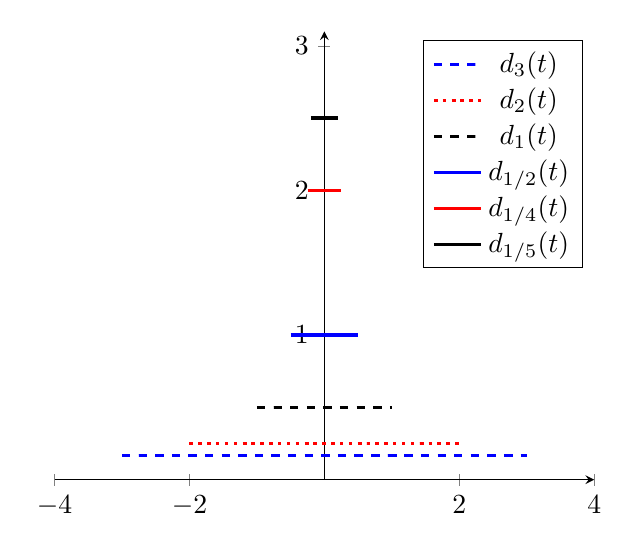
\begin{tikzpicture}
            \begin{axis}[axis lines=center, xmin=-4, xmax=4, ymin=0, ymax=3.1]
                \addplot[smooth, blue, very thick, domain=-3:3, dashed] {0*x+1/6};
                \addlegendentry{$d_3(t)$};
                \addplot[smooth, red, very thick, domain=-2:2, dotted] {0*x+1/4};
                \addlegendentry{$d_2(t)$};
                \addplot[smooth, black, very thick, domain=-1:1, dashed] {0*x+1/2};
                \addlegendentry{$d_1(t)$};
                \addplot[smooth, blue, very thick, domain=-0.5:0.5] {0*x+1/1};
                \addlegendentry{$d_{1/2}(t)$};
                \addplot[smooth, red, very thick, domain=-.25:.25] {0*x+1/0.5};
                \addlegendentry{$d_{1/4}(t)$};
                \addplot[smooth, black, very thick, domain=-.2:.2] {0*x+1/0.4};
                \addlegendentry{$d_{1/5}(t)$};
            \end{axis}
        \end{tikzpicture}
    \end{center}
    \caption{The function $d_k(t)$ for several values of $k$.  In this limit this
    function approximates the Dirac delta function.}
    \label{fig:delta_approx}
\end{figure}

% \begin{problem}
%     Consider the function 
%     \[ d_k(t) = \left\{ \begin{array}{cc} \frac{1}{2k}, & \text{ if } -k \le t \le k \\ 0, &
%         \text{ otherwise} \end{array} \right. \]
%     and observe that
%     \[ \lim_{k \to \infty} d_k(t) = \left\{ \begin{array}{cc} 0, & \text{ if } t \neq a \\
%             \infty, & \text{ if } t=a \end{array} \right. \]
%     where for every $k$ we must have
%     \[ \int_{-\infty}^\infty d_k(t) dt = 1. \]
%     \begin{enumerate}
%         \item[(a)] Write the integral for $\lap{d_k(t-c)}$ where $c$ is a positive shift
%             (centering the function at $t=c$).
%             \solution{
%                 \[ \lap{d_k(t-c)} = \int_0^\infty e^{-st} d_k(t-c) dt = \int_{k-c}^{k+c}
%                     \frac{1}{2k} e^{-st} dt = \frac{1}{2k} \int_{k-c}^{k+c} e^{-st} dt =
%                     \frac{-1}{2ks} e^{-st} \Big|_{t=k-c}^{t=k+c}  \]
%             }
%     \end{enumerate}
% \end{problem}
% 
% 
% \begin{center}
%         FINISH THIS SECTION
% \end{center}
% To answer this question we will look at a slightly more technical definition of the
% Laplace transform:
% \begin{flalign}
%     \lap{f(t)} = \int_{0^-}^\infty e^{-st} f(t) dt.
%     \label{eqn:laplace_technical_defn}
% \end{flalign}
% In \eqref{eqn:laplace_technical_defn} we see that the lower bound of the integral is
% actually the value as we approach 0 from the left.  We didn't define the Laplace transform
% in this way before since it wasn't necessary and didn't change any of our results.
% Equation \eqref{eqn:laplace_technical_defn} {\it is} the correct definition of the Laplace
% transform.
% 
% Applying \eqref{eqn:laplace_technical_defn} to the delta function centered at $t=0$ gives the following:
% \begin{flalign*}
%     \lap{\delta(t)} &= \int_{0^-}^\infty e^{-st} \delta(t) dt.
% \end{flalign*}
% Using integration by parts with $u=e^{-st}$ and $dv = \delta(t)$ we see that $du =
% -se^{-st}dt$ and $v = u_0(t)$ (the Heaviside function with a jump at zero \ldots and yes,
% the notation is unfortunate here).  Hence
% \begin{flalign*}
%     \lap{\delta(t)} &= e^{-st} u_0(t) \Big|_{t\to 0^-}^{t\to\infty} - \int_{0^-}^\infty
%     -se^{-st} u_0(t) dt \\
%     &= 0 + s \int_{0^-}^\infty e^{-st} dt \\
%     &= \frac{s}{-s} e^{-st} \Big|_{t \to 0^-}^{t\to\infty} \\
%     &= -1(0-1) = 1.
% \end{flalign*}
% \begin{thm}
%     The Laplace transform of the Dirac delta function $\delta(t)$ is 
%     \[ \lap{\delta(t)} = 1. \]
% \end{thm}
% 
% If we apply a shift to the delta function and then take the Laplace transform we get
% \[ \lap{\delta_c(t)} = \
% 
% 

This is all well and good, but what is the Laplace transform of the Dirac delta function?
To answer this question we explore one more property of the delta function
\begin{flalign}
    \int_{-\infty}^\infty \delta_a(t) f(t) dt  = f(a). \label{eqn:delta_function_eval}
\end{flalign}
In words, \eqref{eqn:delta_function_eval} says that if we take the product of the delta
function and a (suitably continuous) function $f(t)$ and integrate over the whole real
line then we simply extract the function value of $f(t)$ located at the spike of the delta
function.  In this sense, the delta function just probes function values. 
\begin{problem}
    Provide a graphical reason why 
    \[ \int_{-\infty}^\infty \delta_a(t) f(t) dt = f(a). \]
\end{problem}
From here we get a simple formula for the Laplace transform of the delta function.  
\[ \lap{\delta_a(t)} = \int_0^\infty e^{-st} \delta_a(t) dt = \int_{-\infty}^\infty
    e^{-st} \delta_a(t) dt = e^{-as}. \]
\begin{thm}[Properties of the Dirac Delta Function]
    Let $\delta_a(t)$ be the shifted Dirac delta function.  The delta function has the
    following properties.
    \begin{flalign*}
        &\delta_a(t) = \left\{ \begin{array}{cc} 0, & \text{ if } t \neq a \\ \infty, &
            \text{ if } t=a \end{array} \right. \\
        &\int_{-\infty}^\infty \delta_a(t) dt = 1 \\
        &\int_{-\infty}^\infty \delta_a(t) f(t) dt = f(a) \\
        &\lap{\delta_a(t)} = e^{-as} \\
        &\lap{\delta_0(t)} = 1
    \end{flalign*}
\end{thm}

To make the inversion of the Laplace transform of the delta function more useful we
finally consider the following theorem.
\begin{thm}\label{thm:laplace_delta_shift}
    Let $f(t)$ be a function where $\lap{f(t)} = F(s)$ exists. 
    \[ \lapinv{e^{-as} F(s)} = u(t-a)f(t-a) = u_a(t) f(t-a). \]
    \[ \lap{u_a(t) f(t-a)} = e^{-as} \lap{f(t)} \]
\end{thm}
For example consider the expression $\frac{e^{-2s}}{s+1}$.  The inverse Laplace transform
of this expression is
\[ \lapinv{\frac{e^{-2s}}{s+3}} = u(t-2) e^{-3(t-2)} = u_2(t) e^{-3(t-2)}. \]

\begin{problem}
    Explain what Theorem \ref{thm:laplace_delta_shift} says and create a few examples of
    this theorem in action.
\end{problem}

\begin{problem}
    Solve the differential equation
    \[ x' + \frac{1}{2} x = \delta_3(t) \]
    with the initial condition $x(0) = 5$. Draw a picture of your solution and explain
    what happened.
\end{problem}
\solution{
    \begin{flalign*}
        &x' + \frac{1}{2} x = \delta_3(t) \\
        &\implies sX - x(0) + \frac{1}{2} X = e^{-3s} \\
        &\implies \left( s+\frac{1}{2} \right)X = 5 + e^{-3s} \\
        &\implies X = \frac{5}{s+1/2} + \frac{e^{-3s}}{s+1/2} \\
        &\implies x(t) = 5e^{-0.5t} + u_3(t) e^{-0.5(t-3)}
    \end{flalign*}
    \begin{center}
        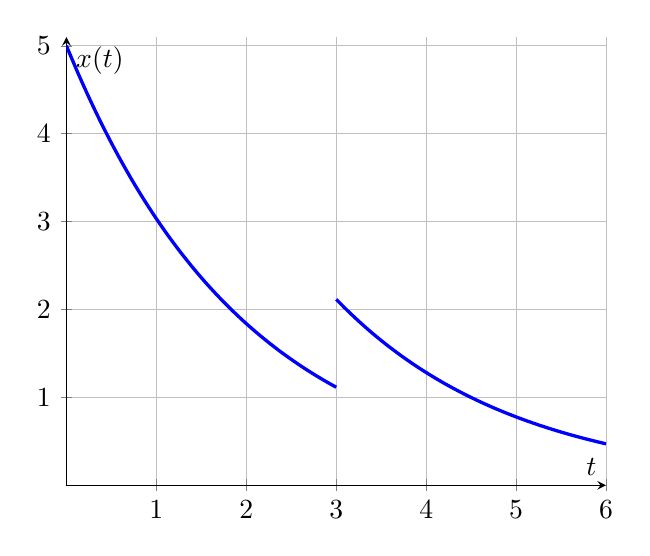
\begin{tikzpicture}
            \begin{axis}[axis lines=center, xmin=0, xmax=6, grid, ymin=0, ymax=5.1,
                xlabel={$t$}, ylabel={$x(t)$}]
                \addplot[smooth, very thick, blue, domain=0:3] {5*exp(-0.5*x)};
                \addplot[smooth, very thick, blue, domain=3:6]
                {5*exp(-0.5*x)+exp(-0.5*(x-3))};
            \end{axis}
        \end{tikzpicture}
    \end{center}
}
\begin{problem}
    Let's return to the differential equation $x' + \frac{1}{2} x = u_3(t)$ with $x(0)
    =5$.  
    \begin{enumerate}
        \item[(a)] Return to your notes from Problem \ref{prob:laplace_ode_shift} and
            recall our conjecture for the plot of the solution.
        \item[(b)] Take the Laplace transform of both sides and rearrange to solve for
            $X(s) = \lap{x(t)}$.
            \solution{
                From Problem \ref{prob:laplace_ode_shift} recall that 
                \[ X(s) = \frac{5}{s+1/2} + \frac{e^{-3s}}{s(s+1/2)} \]
                Using the idea of partial fraction we can rewrite the second fraction as
                \[ \frac{e^{-3s}}{s(s+1/2)} = \frac{Ae^{-3s}}{s} + \frac{Be^{-3s}}{s+1/2} \]
                so if we cancel the $e^{-3s}$ from both sides and clear the fractions we
                get
                \[ 1 = A(s+1/2) + Bs \]
                which means that $A = 2$ and $B = -2$.  Therefore,
                \[ X(s) = \frac{5}{s+1/2} + 2\frac{e^{-3s}}{s} - 2\frac{e^{-3s}}{s+1/2} \]
            }
        \item[(c)] Take the inverse Laplace transform now with the help of Theorem
            \ref{thm:laplace_delta_shift}.
            \solution{
            The first term inverts to $5e^{-(1/2)t}$.\\
            The second term inverts to $2u_3(t)$ \\
            The third term inverts to $-2u_3(t) e^{-(1/2)(t-2)}$
            }
        \item[(d)] Use MATLAB to create a plot of the solution.  \\ Hint: the Heaviside
            function is the \mcode{heaviside} command in MATLAB.
            \solution{\\
                \texttt{t = 0:0.001:15;}\\
                \texttt{x1 = 5*exp(-(1/2)*t);}\\
                \texttt{x2 = 2*heaviside(t-2);}\\
                \texttt{x3 = -2*heaviside(t-2).*exp(-(1/2)*(t-2));}\\
                \texttt{plot(t,x1+x2+x3)}
                \begin{center}
                    \begin{tikzpicture}
                        \begin{axis}[axis lines=center, xmin=0, xmax=8, ymin=0, ymax=5]
                            \addplot[smooth, very thick, blue, domain=0:2]
                            {5*exp(-0.5*x)};
                            \addplot[smooth, very thick, blue, domain=2:8]
                            {5*exp(-0.5*x)+2-2*exp(-0.5*(x-2))};
                        \end{axis}
                    \end{tikzpicture}
                \end{center}
}
    \end{enumerate}
\end{problem}



\begin{problem}
    Find the Laplace transform of
    \[ f(t) = \left\{ \begin{array}{cc} 0, & t < 3 \\ (t-3)^2, & t \ge 3 \end{array} \right.
    \]
\end{problem}

\begin{problem}
    Find the Laplace transform of
    \[ f(t) = u_5(t) e^{-(t-5)}. \]
\end{problem}
\solution{
    \[ \lap{u_5(t) e^{-(t-5)}} = \frac{e^{-5s}}{s+1} \]
}

\begin{problem}
    Find $\lapinv{\frac{e^{-3s}}{s+2}}$
\end{problem}
\solution{
    \[ \lapinv{\frac{e^{-3s}}{s+2}} = u_3(t) e^{-2(t-3)} \]
}



\begin{problem}
    We have a system modeled as an undamped harmonic oscillator that begins at equilibrium
    and at rest, so $y(0) = y'(0) = 0$.  The systems receives a unit impulse force at $t=4$ so
    that it is modeled by the differential equation
    \[ y'' + 9y = \delta_4(t). \]
    Find $y(t)$.
\end{problem}
\solution{
    \[ y(t) = u_4(t) \sin(3(t-4)). \]
}

\begin{problem}
    Create a differential equation that can only be solved analytically using Laplace
    transforms.  Be sure to provide sufficient initial conditions.  After you've written
    your problem trade with another group and solve the other group's problem.
\end{problem}
\solution{
    Any linear differential equation that contains heaviside or delta functions will work.
}   


\newpage\section{Convolutions (INCOMPLETE)}
\ldots in this section we talk about convolutions \ldots later



\newpage\section{Additional Exercises}



\begin{problem}
    Use Laplace transforms to show that the solution to the differential equation
    \[ x'' + 6x' + 18x = \cos(2t) \quad \text{with} \quad x(0) = 1 \quad \text{and} \quad x'(0) =
    -1 \]
    is
    \[ x(t) = \frac{7}{170} \cos(2t) + \frac{3}{85} \sin(2t) + e^{-3t} \left(
        \frac{163}{170} \cos(3t) + \frac{307}{510} \sin(3t)
    \right) \]
\end{problem}

\begin{problem}
    Solve the differential equation
    \[ y'' +4y' + 13y = \delta_3(t)  \quad \text{with} \quad y(0)=1 \quad \text{and} \quad
    y'(0) =0. \]
    Before solving the differential equation sketch a graph of what the homogeneous
    solution looks like and then modify it to account for the delta function.
\end{problem}



\begin{problem}\label{prob:laplace_drug}
    An oral drug is given in periodic doses with the first dose being 2mg.  The person's
        metabolism is such that half of the drug is left in the body after 5 hours.  At every 5
        hour mark another dose of the drug is given.  
        \begin{enumerate}
            \item[(a)] Fill in the blanks for the differential equation where $D$ is the dose (in mg)
                and $t$ is the time (in hours).
                \[ \frac{dD}{dt} = -k_1 \underline{\hspace{0.75in}} + k_2 \underline{\hspace{0.75in}}
                + k_3 \underline{\hspace{0.75in}} + k_4 \underline{\hspace{0.75in}} + \cdots. \]
                The first blank correponds to the way that the drug is removed from the
                system, the second blank
                corresponds to the dose at 5 hours, the third blank corresponds to the
                dose at 10 hours, etc.
            \item[(b)] Use Laplace Transforms to solve your differential equation.
            \item[(c)] Find the constant $k_1$ from the initial information.  
            \item[(d)] Find the constants $k_2, k_3, \dots$ by assuming that right after each
                dose the amount in the patient's system jumps back to 2.
        \end{enumerate}
\end{problem}


\begin{problem}
    In Problem \ref{prob:laplace_drug} we build a differential equation for a drug dosing
    problem.  The trouble with the model built in that problem is that it doesn't account
    for the time that it takes for the drug to go from the stomach to the blood stream.
    Instead, consider the following system of differential equations.
    \begin{flalign*}
        \frac{dS}{dt} &= -C S + k_2 \delta(t-5) + k_3 \delta(t-10) + k_4 \delta(t-15) +
        \cdots \\
        \frac{dB}{dt} &= CS - k_1 B
    \end{flalign*}
    where $S(t)$ is the amount of drug in the stomach and $B(t)$ is the amount of drug in
    the blood stream at time $t$.  
    \begin{enumerate}
        \item[(a)] Explain each term in the model.  Notice that the sum of the two models
            gives us exactly the same model that we had in Problem
            \ref{prob:laplace_drug}.
        \item[(b)] We will now analyze this system of differential equations numerically
            since we don't have all of the tools to solve a system with Laplace
            transforms (\dots so much math but only finite time \dots).  We will use the
            same values of $k_1, k_2, \dots$ for this problem.  We need a constant for $C$
            (the rate at which the drug moves from the stomach to the blood stream) so at
            first pass let's just use $C = 0.1$.

            Complete the following block of code to build an Euler solver for the system
            of differential equations.  When the code is complete, run it to verify that
            what you see has the correct qualitative solution based on your understanding
            of basic biology.  What is wrong with the new model?  What is better aboud the
            new model? How would we improve the downsides to this model?
    \end{enumerate}
\end{problem}

\begin{lstlisting}
clear; clc;
k1 =  % fill in this line with the value of k1 from the prev. problem
C = 0.1;
dt = 0.01;
t = 0:dt:40;
Stomach = zeros(length(t),1);
Blood = zeros(length(t),1);
Stomach(1) = 2; % initial condition
Blood(1) = 0; % initial condition
for n=1:length(t)-1
    if mod(t(n),5) == 0 && t(n)>0
        Stomach(n+1) = Stomach(n) + dt*(-C*Stomach(n)) + 1; % what does this do
    else
        Stomach(n+1) = Stomach(n) + dt*( ... ) % finish the Euler solver
    end
    Blood(n+1) = Blood(n) + dt*( ...  ) % finish the Euler solver
end
plot(t,Stomach,'b',t,Blood,'r')
\end{lstlisting}


